\section{\textbf{Binary Erasure Channel}}
\subsection{Introduction}
\begin{frame}{Binary Erasure Channel(BEC)}
\;\;\;\;\;\;\;\;The binary erasure channel (BEC) models a memoryless channel with two inputs \{0, 1\} andthree outputs, \{0, 1, ?\}, where “?” is an “erasure symbol.” The probability that any transmitted
bit will be received correctly is 1 - p, that it will be erased is p, and that it will be received
incorrectly is zero. These transition probabilities are summarized in Figure  below.  
\begin{alertblock}{Transition probabilities of the binary erasure channel}
\begin{figure}
			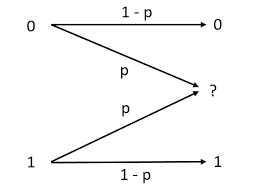
\includegraphics[width=6cm, height=3cm]{BEC/bec pic.png}
			\label{bec}
\end{figure}
\end{alertblock}
\end{frame}
\subsection{Iterative decoding of LDPC codes on the BEC}
\begin{frame}{Iterative decoding of LDPC codes on the BEC}
\;\;\;\;\;\;On the binary erasure channel, the sum-product algorithm is greatly simplified, because at any
time every variable corresponding to every edge in the code graph is either known perfectly
(unerased) or not known at all (erased). Iterative decoding using the sum-product algorithm
therefore reduces simply to the propagation of unerased variables through the code graph.\\~\\
\;\;\;\;\;\;There are only two types of nodes in a normal graph of an LDPC code repetition nodes and zero-sum nodes. If all variables are either correct or erased, then the
sum-product update rule for a repetition node reduces simply to:\\~\\
\;\;\;\;\;\;$\bullet$ If any incident variable is unerased, then all other incident variables may be set equal to that variable, with complete confidence; otherwise, all incident variables remain erased.\\~\\
For a zero-sum node, the sum-product update rule reduces to:\\~\\
\;\;\;\;\;\;$\bullet$ If all but one incident variable is unerased, then the remaining incident variable may
be set equal to the mod-2 sum of those inputs, with complete confidence; otherwise,
variable assignments remain unchanged.
\end{frame}
\begin{frame}{Iterative decoding of LDPC codes on the BEC(cont...)}
  Since all unerased variables are correct, there is no chance that these rules could produce a
variable assignment that conflicts with another assignment.\\~\\

\subsection{Results}
\begin{alertblock}{Terminal output}
   \begin{figure}
       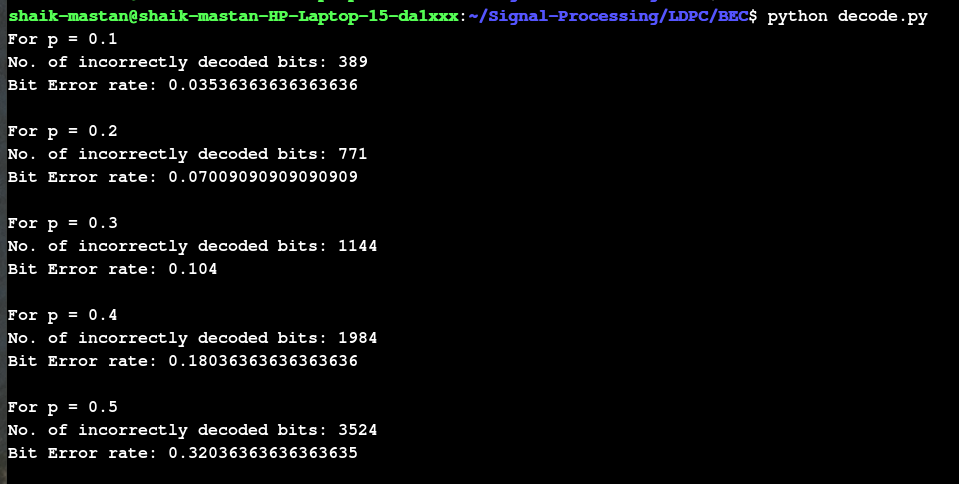
\includegraphics[width = 0.9\textwidth]{BEC/terminalBEC.png}
   \end{figure}
\end{alertblock}
\end{frame}

\begin{frame}
\begin{alertblock}{Plot}
   \begin{figure}
       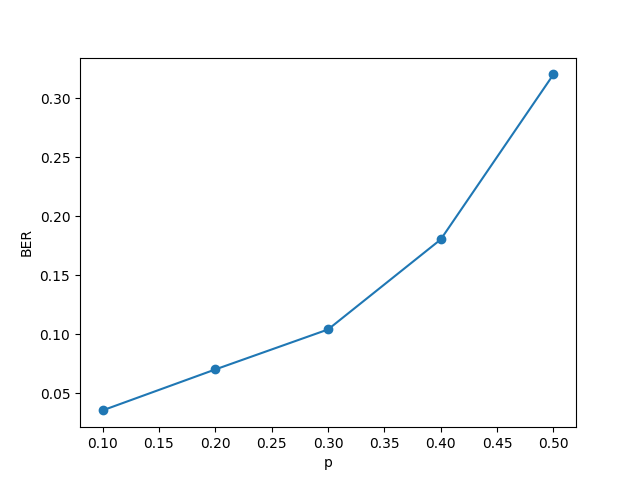
\includegraphics[width = 0.8\textwidth]{BEC/BEC.png}
   \end{figure}
  \end{alertblock}
\end{frame}